\documentclass[a4paper,12pt]{article}

\usepackage[utf8x]{inputenc}
\usepackage[T2A]{fontenc}
\usepackage[english, russian]{babel}

% Опционно, требует  apt-get install scalable-cyrfonts.*
% и удаления одной строчки в cyrtimes.sty
% Сточку не удалять!
% \usepackage{cyrtimes}

% Картнки и tikz
\usepackage{graphicx}
\usepackage{tikz}
\usetikzlibrary{snakes,arrows,shapes}


% Некоторая русификация.
\usepackage{misccorr}
\usepackage{indentfirst}
\renewcommand{\labelitemi}{\normalfont\bfseries{--}}

% Увы, поля придётся уменьшить из-за листингов.
\topmargin -1cm
\oddsidemargin -0.5cm
\evensidemargin -0.5cm
\textwidth 17cm
\textheight 24cm

\sloppy

% Оглавление в PDF
\usepackage[
bookmarks=true,
colorlinks=true, linkcolor=black, anchorcolor=black, citecolor=black, menucolor=black,filecolor=black, urlcolor=black,
unicode=true
]{hyperref}

% Для исходного кода в тексте
\newcommand{\Code}[1]{\texttt{#1}}

\usepackage{verbatim}
\usepackage{fancyvrb}
\fvset{frame=leftline, fontsize=\small, framerule=0.4mm, rulecolor=\color{darkgray}, commandchars=\\\{\}}
\renewcommand{\theFancyVerbLine}{\small\arabic{FancyVerbLine}}


\title{Отчёт по лабораторной работе \\ <<Динамическая IP-маршрутизация>> \\ Вариант №6}
\author{(Овчинников Владислав Александрович)}

\begin{document}

\maketitle

\tableofcontents

\section{Настройка сети}

\subsection{Топология сети}

Топология сети и используемые IP-адреса показаны на рисунке~\ref{fig:network}.

\begin{figure}
\centering
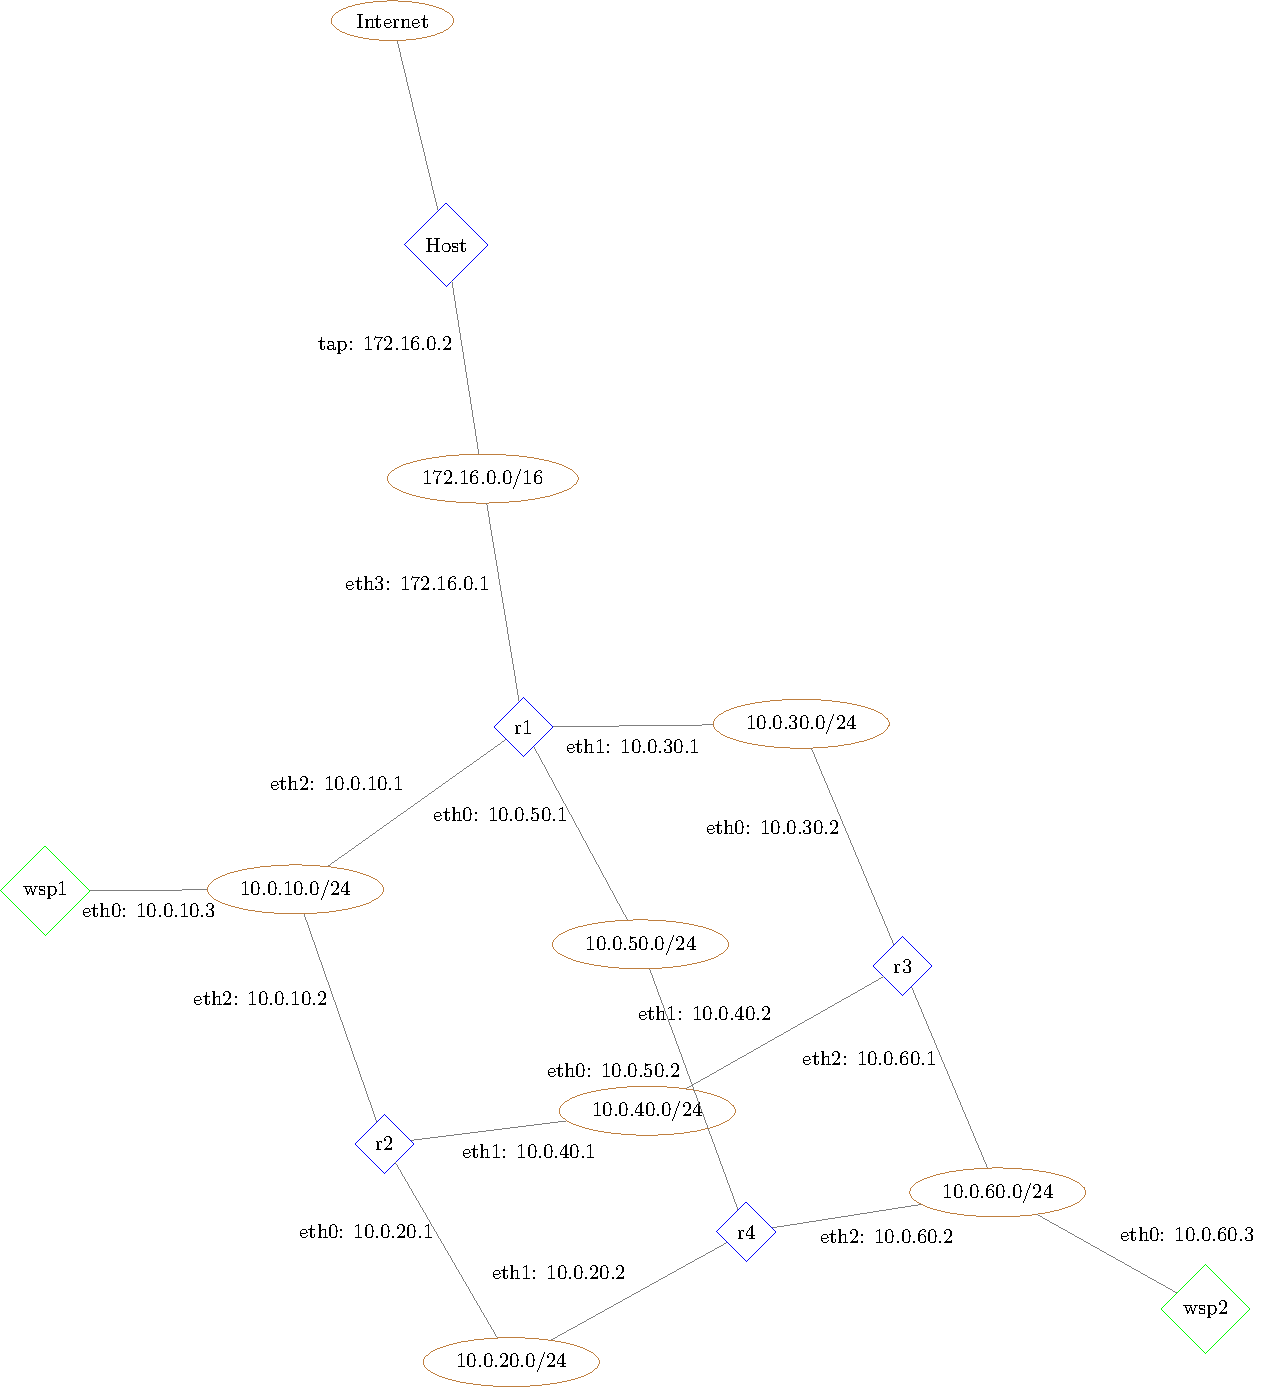
\includegraphics[width=0.8\textwidth]{includes/network_gv.pdf}
\caption{Топология сети}
\label{fig:network}
\end{figure}

Динамическая маршрутизация используется на всех узлах сети, так как все узлы подключены к сегментам сети, к которым подключены более чем один маршрутизатор. Таким образом, перечень узлов, на которых используется динамическая IP-маршрутизация: r1, r2, r3, r4, wsp1, wsp2.

\newpage

\subsection{Назначение IP-адресов}

Для настройки сетевых интерфейсов и присвоения им соответствующих IP-адресов были изменены файлы \textbf{/etc/network/interfaces} соответствующих узлов.

Ниже приведён файл сетевой настройки маршрутизатора \textbf{r1}:

\begin{Verbatim}
auto lo
iface lo inet loopback

auto eth0
iface eth0 inet static
address 10.0.50.1
netmask 255.255.255.0

auto eth1
iface eth1 inet static
address 10.0.30.1
netmask 255.255.255.0

auto eth2
iface eth2 inet static
address 10.0.10.1
netmask 255.255.255.0
\end{Verbatim}

Ниже приведён файл сетевой настройки маршрутизатора \textbf{r2}:

\begin{Verbatim}
auto lo
iface lo inet loopback

auto eth0
iface eth0 inet static
address 10.0.20.1
netmask 255.255.255.0

auto eth1
iface eth1 inet static
address 10.0.40.1
netmask 255.255.255.0

auto eth2
iface eth2 inet static
address 10.0.10.2
netmask 255.255.255.0
\end{Verbatim}

Ниже приведён файл сетевой настройки маршрутизатора \textbf{r3}:

\begin{Verbatim}
auto lo
iface lo inet loopback

auto eth0
iface eth0 inet static
address 10.0.30.2
netmask 255.255.255.0

auto eth1
iface eth1 inet static
address 10.0.40.2
netmask 255.255.255.0

auto eth2
iface eth2 inet static
address 10.0.60.1
netmask 255.255.255.0
\end{Verbatim}

Ниже приведён файл сетевой настройки маршрутизатора \textbf{r4}:

\begin{Verbatim}
auto lo
iface lo inet loopback

auto eth0
iface eth0 inet static
address 10.0.50.2
netmask 255.255.255.0

auto eth1
iface eth1 inet static
address 10.0.20.2
netmask 255.255.255.0

auto eth2
iface eth2 inet static
address 10.0.60.2
netmask 255.255.255.0
\end{Verbatim}

Ниже приведён файл сетевой настройки рабочей станции \textbf{wsp1}.

\begin{Verbatim}
auto lo
iface lo inet loopback

auto eth0
iface eth0 inet static
address 10.0.10.3
netmask 255.255.255.0
\end{Verbatim}

Ниже приведён файл сетевой настройки рабочей станции \textbf{wsp2}.

\begin{Verbatim}
auto lo
iface lo inet loopback

auto eth0
iface eth0 inet static
address 10.0.60.3
netmask 255.255.255.0
\end{Verbatim}


\subsection{Настройка протокола RIP}

\textbf{Quagga} - пакет свободного программного обеспечения, поддерживающий протоколы динамической маршрутизации IP. Компьютер с установленным и сконфигурированным пакетом Quagga способен поддерживать множество протоколов динамической маршрутизации, одним из которых является \textbf{Routing Information Protocol (RIP)}.

\textbf{Протокол маршрутной информации} (Routing Information Protocol - RIP) - один из самых простых протоколов маршрутизации. Применяется в небольших компьютерных сетях, позволяет маршрутизаторам динамически обновлять маршрутную информацию (направление и дальность в хопах), получая ее от соседних маршрутизаторов.

RIP - протокол дистанционно-векторной маршрутизации, который оперирует транзитными участками (хоп) в качестве метрики маршрутизации. Максимальное количество транзитных участков, разрешенное в RIP - 15 (метрика 16 означает "бесконечно большую метрику"). Каждый RIP-маршрутизатор по умолчанию вещает в сеть свою полную таблицу маршрутизации раз в 30 секунд, довольно сильно нагружая низкоскоростные линии связи. В современных сетевых средах RIP - не самое лучшее решение для выбора в качестве протокола маршрутизации, так как его возможности уступают более современным протоколам, таким как EIGRP, OSPF. Ограничение на 15 транзитных участков не дает применять его в больших сетях. Преимущество этого протокола - простота конфигурирования.

В протоколе RIP маршрутизаторы узнают о сетях назначения от соседних маршрутизаторов через процесс совместного использования. Маршрутизаторы, работающие по протоколу RIP, периодически транслируют настроенные сети со всех портов. Список маршрутизаторов обновит их таблицу маршрутизации на основе этой информации.

Иногда RIP также известен как маршрутизация прослушки, потому что в этом протоколе маршрутизации маршрутизаторы изучают информацию о маршрутизации от непосредственно подключенных соседей, а эти соседи учатся от других соседних маршрутизаторов.

Протокол RIP будет совместно использовать настроенные маршруты в сети через широковещательные передачи. Эти широковещательные передачи называются обновлениями маршрутизации. Прослушивающие маршрутизаторы обновят свою таблицу маршрутизации на основе этих обновлений.

Маршрутизатор выполняет несколько измерений, обрабатывая и помещая новую информацию о маршруте в таблицу маршрутизации. Если маршрутизатор обнаружит новый маршрут в обновлении, он поместит его в таблицу маршрутизации.

Через 10 секунд (интервал рассылки заданный в лабораторной работе) все маршрутизаторы снова будут транслировать свои таблицы маршрутизации с обновленной информацией.

Через 10 секунд маршрутизаторы снова будут транслировать новую информацию о маршрутизации. На этот раз маршрутизаторам нечего обновлять. Эта стадия называется конвергенцией.

Конвергенция - это термин, который относится к времени, затраченному всеми маршрутизаторами на понимание текущей топологии сети.

Может быть два или более путей до целевой сети. В этой ситуации RIP использует измерение, называемое метрикой, чтобы определить наилучший путь до целевой сети. RIP использует подсчет прыжков как метрику. Прыжки - это количество маршрутизаторов, необходимое для достижения целевой сети.

Так как в данной сети четыре маршрутизатора и две рабочии станции, которые связаны с несколькими маршрутизаторами, требовалось сконфигурировать RIP на всех узлах сети.

Маршрутизатор \textbf{r1} был выбран для соединения с интернетом. В связи с этим в файле \textbf{lab.conf} для него были произведены первоначальные настройки интерфейса:

\begin{Verbatim}
r1[3]=tap,172.16.0.2,172.16.0.1
\end{Verbatim}

Таким образов, интерфейсу \textbf{eth3} будет присвоен адрес \textbf{172.16.0.1}, а реальной машине присвоен адрес \textbf{172.16.0.2}. Также на этом марштуризаторе в файле \textbf{/etc/rc.local} была включена трансляция ("маскарад") сетевых адресов для пакетов, проходящих через интерфейс \textbf{eth3}:

\begin{Verbatim}
iptables -t nat -A POSTROUTING -o eth3 -j MASQUERADE
\end{Verbatim}

Также для данного маршрутизатора было отключено распространение им по протоколу RIP информации о сети \textbf{172.16.0.0/16}. Для этого был закомментирована в файле \textbf{/etc/quagga/ripd.conf} строка \textbf{redistribute connected}.

В заключении настройки данного маршрутизатора были добавлены интерфейсы в файл \textbf{/etc/quagga/ripd.conf}, через которые следует рассылать и принимать сообщения протокола RIP. Таким образом, были добавлены все интерфейсы, кроме \textbf{eth3}, по причине того, что не требуется в виртуальной сети знать информацию о сегменте сети \textbf{172.16.0.0/16}.

Ниже приведен файл \Code{/etc/quagga/ripd.conf} маршрутизатора \textbf{r1}:

\begin{Verbatim}
router rip

network eth0
network eth1
network eth2

timers basic 10 60 120

redistribute kernel

log file /var/log/quagga/ripd.log
\end{Verbatim}

Ниже приведен файл \Code{/etc/quagga/ripd.conf} маршрутизатора \textbf{r2}:

\begin{Verbatim}
router rip

network eth0
network eth1
network eth2

timers basic 10 60 120

redistribute kernel
redistribute connected

log file /var/log/quagga/ripd.log
\end{Verbatim}

Ниже приведен файл \Code{/etc/quagga/ripd.conf} маршрутизатора \textbf{r3}:

\begin{Verbatim}
router rip

network eth0
network eth1
network eth2

timers basic 10 60 120

redistribute kernel
redistribute connected

log file /var/log/quagga/ripd.log
\end{Verbatim}

Ниже приведен файл \Code{/etc/quagga/ripd.conf} маршрутизатора \textbf{r4}:

\begin{Verbatim}
router rip

network eth0
network eth1
network eth2

timers basic 10 60 120

redistribute kernel
redistribute connected

log file /var/log/quagga/ripd.log
\end{Verbatim}

Ниже приведен файл \Code{/etc/quagga/ripd.conf} рабочей станции \textbf{wsp1}, связанной с несколькими маршрутизаторам:

\begin{Verbatim}
router rip

network eth0

timers basic 10 60 120

redistribute kernel
redistribute connected

log file /var/log/quagga/ripd.log
\end{Verbatim}

Ниже приведен файл \Code{/etc/quagga/ripd.conf} рабочей станции \textbf{wsp2}, связанной с несколькими маршрутизаторам:

\begin{Verbatim}
router rip

network eth0

timers basic 10 60 120

redistribute kernel
redistribute connected

log file /var/log/quagga/ripd.log
\end{Verbatim}


\section{Проверка настройки протокола RIP}

Требовалось проверить правильность конфигурации RIP. Для этого был произведен вывод пути с помощью \textbf{traceroute}.

Вывод \textbf{traceroute} от узла \textbf{wsp1} до узла \textbf{wsp2} при нормальной работе сети:

\begin{Verbatim}
traceroute to 10.0.60.3 (10.0.60.3), 64 hops max, 40 byte packets
 1  10.0.10.2 (10.0.10.2)  0 ms  0 ms  0 ms
 2  10.0.40.2 (10.0.40.2)  0 ms  0 ms  0 ms
 3  10.0.60.3 (10.0.60.3)  1 ms  1 ms  1 ms
\end{Verbatim}

Вывод \textbf{traceroute} от узла \textbf{wsp2} до внешнего IP \textbf{8.8.8.8}:

\begin{Verbatim}
traceroute to 8.8.8.8 (8.8.8.8), 64 hops max, 40 byte packets
 1  10.0.60.1 (10.0.60.1)  1 ms  1 ms  1 ms
 2  10.0.50.1 (10.0.50.1)  1 ms  1 ms  1 ms
 3  172.16.0.2 (172.16.0.2)  1 ms  1 ms  1 ms
 4  192.168.0.1 (192.168.0.1)  3 ms  2 ms  2 ms
 5  90.154.77.227 (90.154.77.227)  9 ms  4 ms  4 ms
 6  * 77.37.250.200 (77.37.250.200)  7 ms  5 ms
 7  * 77.37.250.249 (77.37.250.249)  5 ms  6 ms
 8  72.14.209.81 (72.14.209.81)  38 ms  28 ms  26 ms
 9  108.170.250.34 (108.170.250.34)  6 ms (TOS=128!) 108.170.250.99 (108.170.250.99)  6 ms  6 ms
10  * 172.253.66.116 (172.253.66.116) [MPLS: Label 24382 Exp 4]  21 ms 216.239.50.46 (216.239.50.46) [MPLS: Label 26247 Exp 4]  21 ms
11  72.14.235.69 (72.14.235.69)  22 ms 108.170.235.204 (108.170.235.204)  22 ms 209.85.254.20 (209.85.254.20)  29 ms
12  108.170.233.163 (108.170.233.163)  27 ms 142.250.56.215 (142.250.56.215)  21 ms 142.250.56.221 (142.250.56.221)  22 ms
13  * * *
14  * * *
15  * * *
16  * * *
17  * * *
18  * * *
19  * * *
20  * * *
21  * * *
22  8.8.8.8 (8.8.8.8)  23 ms  21 ms *
\end{Verbatim}

Также для проверки RIP были перехвачены датаграммы UDP с помощью \textbf{tcpdump}.

Вывод сообщения RIP, перехваченного на маршрутизаторе \textbf{r4}:

\begin{Verbatim}
IP (tos 0x0, ttl 1, id 0, offset 0, flags [DF], proto UDP (17), length 132) 10.0.50.1.520 > 224.0.0.9.520: 
	RIPv2, Response, length: 104, routes: 5
	  AFI: IPv4:       10.0.10.0/24, tag 0x0000, metric: 1, next-hop: self
	  AFI: IPv4:       10.0.20.0/24, tag 0x0000, metric: 2, next-hop: self
	  AFI: IPv4:       10.0.30.0/24, tag 0x0000, metric: 1, next-hop: self
	  AFI: IPv4:       10.0.40.0/24, tag 0x0000, metric: 2, next-hop: self
	  AFI: IPv4:       10.0.60.0/24, tag 0x0000, metric: 2, next-hop: self
\end{Verbatim}

Вывод таблицы RIP на маршрутизаторе \textbf{r4}:

\begin{Verbatim}
     Network            Next Hop         Metric From            Tag Time
R(n) 0.0.0.0/0          10.0.50.1             2 10.0.50.1         0 00:58
R(n) 10.0.10.0/24       10.0.20.1             2 10.0.20.1         0 00:55
C(i) 10.0.20.0/24       0.0.0.0               1 self              0
R(n) 10.0.30.0/24       10.0.50.1             2 10.0.50.1         0 00:58
R(n) 10.0.40.0/24       10.0.20.1             2 10.0.20.1         0 00:55
C(i) 10.0.50.0/24       0.0.0.0               1 self              0
C(i) 10.0.60.0/24       0.0.0.0               1 self              0
\end{Verbatim}

Вывод таблицы маршрутизации на маршрутизаторе \textbf{r4}:

\begin{Verbatim}
10.0.20.0/24 dev eth1  proto kernel  scope link  src 10.0.20.2 
10.0.50.0/24 dev eth0  proto kernel  scope link  src 10.0.50.2 
10.0.60.0/24 dev eth2  proto kernel  scope link  src 10.0.60.2 
10.0.30.0/24 via 10.0.50.1 dev eth0  proto zebra  metric 2 
10.0.40.0/24 via 10.0.20.1 dev eth1  proto zebra  metric 2 
10.0.10.0/24 via 10.0.20.1 dev eth1  proto zebra  metric 2 
default via 10.0.50.1 dev eth0  proto zebra  metric 2
\end{Verbatim}

\section{Расщепленный горизонт и испорченные обратные обновления}

Split horizon (расщепленный горизонт) - это механизм, который утверждает, что, если маршрутизатор получает обновление для маршрута на любом интерфейсе, он не будет передавать ту же информацию о маршруте обратно маршрутизатору-отправителю на том же порту. Расщепленный горизонт используется для того, чтобы избежать циклов маршрутизации.

Маршрут отравления (испорченные обновления) - маршрут отравления работает в противоположном режиме расщепленного горизонта. Когда маршрутизатор замечает, что какой-либо из его непосредственно подключенных маршрутизатов вышел из строя, он отправляет этот маршрут. По умолчанию пакет может путешествовать только 15 прыжков RIP. Любой маршрут за пределами 15 прыжков является недопустимым маршрутом для RIP. В маршруте, находящемся в неисправном состоянии, RIP присваивает значение выше 15 к конкретному маршруту. Эта процедура известна как маршрутное отравление. Отравленный маршрут будет транслироваться со всех активных интерфейсов. Принимающий сосед будет игнорировать правило расщепления горизонта, передавая тот же отравленный маршрут обратно отправителю. Этот процесс гарантирует, что каждый маршрутизатор обновит информацию об отравленном маршруте.

Опыты с расщепленным горизонтом и испорченными обратными обновлениями проводились на маршрутизаторе \textbf{r4}.

Вывод сообщений на маршрутизаторе \textbf{r4} с включенным расщепленным горизонтом и с включенными испорченными обновлениями:

\begin{Verbatim}
IP (tos 0x0, ttl 1, id 0, offset 0, flags [DF], proto UDP (17), length 172) 10.0.50.2.520 > 224.0.0.9.520: 
	RIPv2, Response, length: 144, routes: 7
	  AFI: IPv4:         0.0.0.0/0 , tag 0x0000, metric: 16, next-hop: 10.0.50.1
	  AFI: IPv4:       10.0.10.0/24, tag 0x0000, metric: 16, next-hop: 10.0.50.1
	  AFI: IPv4:       10.0.20.0/24, tag 0x0000, metric: 1, next-hop: self
	  AFI: IPv4:       10.0.30.0/24, tag 0x0000, metric: 16, next-hop: 10.0.50.1
	  AFI: IPv4:       10.0.40.0/24, tag 0x0000, metric: 2, next-hop: self
	  AFI: IPv4:       10.0.50.0/24, tag 0x0000, metric: 16, next-hop: self
	  AFI: IPv4:       10.0.60.0/24, tag 0x0000, metric: 1, next-hop: self
\end{Verbatim}

Можно заметить, что метрику \textbf{16} получили сети \textbf{10.0.50.0/24}, \textbf{10.0.30.0/24}, \textbf{10.0.10.0/24}, \textbf{0.0.0.0/0}.

Вывод сообщений на маршрутизаторе \textbf{r4} с выключенным расщепленным горизонтом:

\begin{Verbatim}
IP (tos 0x0, ttl 1, id 0, offset 0, flags [DF], proto UDP (17), length 172) 10.0.50.2.520 > 224.0.0.9.520: 
	RIPv2, Response, length: 144, routes: 7
	  AFI: IPv4:         0.0.0.0/0 , tag 0x0000, metric: 2, next-hop: 10.0.50.1
	  AFI: IPv4:       10.0.10.0/24, tag 0x0000, metric: 2, next-hop: 10.0.50.1
	  AFI: IPv4:       10.0.20.0/24, tag 0x0000, metric: 1, next-hop: self
	  AFI: IPv4:       10.0.30.0/24, tag 0x0000, metric: 2, next-hop: 10.0.50.1
	  AFI: IPv4:       10.0.40.0/24, tag 0x0000, metric: 2, next-hop: self
	  AFI: IPv4:       10.0.50.0/24, tag 0x0000, metric: 1, next-hop: self
	  AFI: IPv4:       10.0.60.0/24, tag 0x0000, metric: 1, next-hop: self
\end{Verbatim}

При включенном расщепленном горизонте и включенных испорченных обновлениях в сообщениях протокола RIP поле next-hop у ряда сетей стало отличаться от самого отправляющего, но это является не важным, так как метрика сети равна 16 и до анализа этого поля получатель сообщения не должен дойти.

При выключенном расщепленном горизонте для ряда сетей, которые были бы исключены при включенном правиле расщепленного горизонта, поле next-hop указывает адрес не самого отправителя, а следующий маршрутизатор на пути к данной сети. Именно значение этого поля соседи должны использовать в качестве следующего, если вдруг их удовлетворит данный маршрут.

\section{Имитация устранимой поломки в сети}

Для имитации устранимой поломки в сети был отключен маршрутизатор \textbf{r3}.

Вывод с помощью \textbf{traceroute} пути от узла \textbf{wsp1} до узла \textbf{wsp2} до отключения маршрутизатора \textbf{r3}:

\begin{Verbatim}
traceroute to 10.0.60.3 (10.0.60.3), 64 hops max, 40 byte packets
 1  10.0.10.1 (10.0.10.1)  1 ms  7 ms  2 ms
 2  10.0.30.2 (10.0.30.2)  2 ms  3 ms  1 ms
 3  10.0.60.3 (10.0.60.3)  2 ms  3 ms  1 ms
\end{Verbatim}

Вывод таблицы RIP непосредственно перед истечением таймера устаревания (на маршрутизаторе-соседе отключенного \textbf{r2}):

\begin{Verbatim}
     Network            Next Hop         Metric From            Tag Time
R(n) 0.0.0.0/0          10.0.10.1             2 10.0.10.1         0 00:57
C(i) 10.0.10.0/24       0.0.0.0               1 self              0
C(i) 10.0.20.0/24       0.0.0.0               1 self              0
R(n) 10.0.30.0/24       10.0.40.2             2 10.0.40.2         0 00:03
C(i) 10.0.40.0/24       0.0.0.0               1 self              0
R(n) 10.0.50.0/24       10.0.20.2             2 10.0.20.2         0 00:51
R(n) 10.0.60.0/24       10.0.20.2             2 10.0.20.2         0 00:51
\end{Verbatim}

Перестроенная таблица на маршрутизаторе \textbf{r2}

\begin{Verbatim}
     Network            Next Hop         Metric From            Tag Time
R(n) 0.0.0.0/0          10.0.10.1             2 10.0.10.1         0 00:53
C(i) 10.0.10.0/24       0.0.0.0               1 self              0
C(i) 10.0.20.0/24       0.0.0.0               1 self              0
R(n) 10.0.30.0/24       10.0.20.2             3 10.0.20.2         0 00:59
C(i) 10.0.40.0/24       0.0.0.0               1 self              0
R(n) 10.0.50.0/24       10.0.20.2             2 10.0.20.2         0 00:59
R(n) 10.0.60.0/24       10.0.20.2             2 10.0.20.2         0 00:59
\end{Verbatim}

Вывод с помощью \textbf{traceroute} от узла \textbf{wsp1} до узла \textbf{wsp2} после того, как служба RIP перестроила таблицы маршрутизации.

\begin{Verbatim}
traceroute to 10.0.60.3 (10.0.60.3), 64 hops max, 40 byte packets
 1  10.0.10.1 (10.0.10.1)  8 ms  0 ms  0 ms
 2  10.0.50.2 (10.0.50.2)  11 ms  0 ms  0 ms
 3  10.0.60.3 (10.0.60.3)  12 ms  0 ms  0 ms
\end{Verbatim}

\section{Имитация неустранимой поломки в сети}

Для имитации неустранимой поломки в сети требовалось отключить \textbf{r3} и \textbf{r4}, что привело к недостижимости узла \textbf{wsp2}.

RIP-таблица на маршрутизаторе \textbf{r2} до отключения маршрутизаторов \textbf{r3} и \textbf{r4}:

\begin{Verbatim}
     Network            Next Hop         Metric From            Tag Time
R(n) 0.0.0.0/0          10.0.10.1             2 10.0.10.1         0 00:54
C(i) 10.0.10.0/24       0.0.0.0               1 self              0
C(i) 10.0.20.0/24       0.0.0.0               1 self              0
R(n) 10.0.30.0/24       10.0.10.1             2 10.0.10.1         0 00:54
C(i) 10.0.40.0/24       0.0.0.0               1 self              0
R(n) 10.0.50.0/24       10.0.10.1             2 10.0.10.1         0 00:54
R(n) 10.0.60.0/24       10.0.40.2             2 10.0.40.2         0 00:04
\end{Verbatim}

Перестроенная RIP-таблица на маршрутизаторе \textbf{r2} после отключения маршрутизаторов \textbf{r3} и \textbf{r4}, где видна 16-ая метрика:

\begin{Verbatim}
     Network            Next Hop         Metric From            Tag Time
R(n) 0.0.0.0/0          10.0.10.1             2 10.0.10.1         0 00:52
C(i) 10.0.10.0/24       0.0.0.0               1 self              0
C(i) 10.0.20.0/24       0.0.0.0               1 self              0
R(n) 10.0.30.0/24       10.0.10.1             2 10.0.10.1         0 00:52
C(i) 10.0.40.0/24       0.0.0.0               1 self              0
R(n) 10.0.50.0/24       10.0.10.1             2 10.0.10.1         0 00:52
R(n) 10.0.60.0/24       10.0.10.1            16 10.0.10.1         0 00:05
\end{Verbatim}

RIP-таблица на рабочей станции \textbf{wsp2} до отключения маршрутизаторов \textbf{r3} и \textbf{r4}:

\begin{Verbatim}
     Network            Next Hop         Metric From            Tag Time
R(n) 0.0.0.0/0          10.0.60.2             3 10.0.60.2         0 00:11
R(n) 10.0.10.0/24       10.0.60.2             3 10.0.60.2         0 00:11
R(n) 10.0.20.0/24       10.0.60.2             2 10.0.60.2         0 00:11
R(n) 10.0.30.0/24       10.0.60.1             2 10.0.60.1         0 00:01
R(n) 10.0.40.0/24       10.0.60.1             2 10.0.60.1         0 00:01
R(n) 10.0.50.0/24       10.0.60.2             2 10.0.60.2         0 00:11
C(i) 10.0.60.0/24       0.0.0.0               1 self              0
\end{Verbatim}

Перестроенная RIP-таблица на рабочей станции \textbf{wsp2} после отключения маршрутизаторов \textbf{r3} и \textbf{r4}, где видна 16-ая метрика:

\begin{Verbatim}
     Network            Next Hop         Metric From            Tag Time
R(n) 0.0.0.0/0          10.0.60.2            16 10.0.60.2         0 01:52
R(n) 10.0.10.0/24       10.0.60.2            16 10.0.60.2         0 01:52
R(n) 10.0.20.0/24       10.0.60.2            16 10.0.60.2         0 01:52
R(n) 10.0.30.0/24       10.0.60.1            16 10.0.60.1         0 01:42
R(n) 10.0.40.0/24       10.0.60.1            16 10.0.60.1         0 01:42
R(n) 10.0.50.0/24       10.0.60.2            16 10.0.60.2         0 01:52
C(i) 10.0.60.0/24       0.0.0.0               1 self              0
\end{Verbatim}

\section{Выводы}

В процессе выполнения данной лабораторной работы были выполнены следующие поставленные задачи:

1. Построена и сконфигурирована сеть в соответствии с поставленным вариантом.

2. Настроены сетевые интерфейсы у виртуальных машин.

3. Сконфигурирован протокол RIP с помощью ПО Quagga и конфигурационного файла /etc/quagga/ripd.conf.

4. Настроен подключения к внешней сети из виртуальных машин и выход в Интернет.

5. Протестирована и проверена настройка динамической маршрутизации и автоматическое заполнение маршрутных таблиц.

6. Проведены опыты с расщепленным горизонтом и испорченным обратным маршрутом.

7. Проведен опыт с устранением поломки в сети (при перестроении маршрута).

8. Проведен опыт, когда невозможно устранить поломку в сети и узел полностью недостижим.

Таким образом, все поставленные задачи были выполнены.

\end{document}
